% ====================================================
% PROVISIONAL PATENT APPLICATION
% Curvature-Guided Wavefront Execution for GPU-CSP
% Bee Rosa Davis (she/her)
% ====================================================
\documentclass[11pt,letterpaper]{article}
\usepackage[margin=1in]{geometry}
\usepackage{amsmath,amssymb,amsfonts,amsthm}
\usepackage{mathtools}
\usepackage{enumitem}
\usepackage{hyperref}
\usepackage{xcolor}
\usepackage{titlesec}
\usepackage{parskip}
\usepackage{fancyhdr}
\usepackage{lastpage}
\usepackage{tikz}
\usetikzlibrary{arrows.meta,positioning,shapes.geometric,calc,fit,backgrounds}
\usepackage{algorithm2e}
\usepackage{booktabs}
\usepackage{longtable}
\usepackage{graphicx}
\graphicspath{{../../visualizations/}}

% Section formatting
\titleformat{\section}{\normalfont\large\bfseries}{\thesection}{1em}{}
\titleformat{\subsection}{\normalfont\normalsize\bfseries}{\thesubsection}{1em}{}
\titleformat{\subsubsection}{\normalfont\normalsize\itshape}{\thesubsubsection}{1em}{}

% Header/footer
\pagestyle{fancy}
\fancyhf{}
\lhead{\footnotesize Provisional Patent Application}
\rhead{\footnotesize Confidential}
\cfoot{\footnotesize \thepage}
\renewcommand{\headrulewidth}{0pt}
\renewcommand{\footrulewidth}{0pt}

% Theorem environments
\newtheorem{definition}{Definition}
\newtheorem{theorem}{Theorem}
\newtheorem{proposition}{Proposition}
\newtheorem{lemma}{Lemma}

\hypersetup{
  colorlinks=true,
  linkcolor=black,
  urlcolor=blue!60!black,
  citecolor=black,
  pdfauthor={Bee Rosa Davis},
  pdftitle={Provisional Patent: Curvature-Guided Wavefront Execution for GPU-Accelerated Constraint Satisfaction}
}

\begin{document}

\begin{center}
\textbf{\Large PROVISIONAL PATENT APPLICATION}
\end{center}

\vspace{1em}

\section*{Title of Invention}

\begin{center}
\textbf{\large SYSTEM AND METHOD FOR CURVATURE-GUIDED WAVEFRONT EXECUTION\\FOR GPU-ACCELERATED CONSTRAINT SATISFACTION\\ON A DISCRETE RIEMANNIAN MANIFOLD}
\end{center}

\vspace{2em}

% ====================================================================
\section*{ABSTRACT}
% ====================================================================

A system and method for solving constraint satisfaction problems (CSPs) on GPU hardware using Riemannian geometric invariants to guide computational resource allocation. The invention computes a local curvature field $K_{\mathrm{loc}}(v)$ over the constraint graph from three independent scalar invariants of a constraint fiber bundle (saturation, scarcity, and coupling norm), derives an information value functional $V(v)$ that subsumes and generalizes classical CSP heuristics (MRV, Degree) as special cases, and uses said functional to order variable resolution for maximum constraint propagation per GPU cycle. A three-phase pipeline (wavefront constraint propagation, continuous manifold relaxation on the probability simplex, curvature-directed speculative branching with holonomy-based pruning) is gated by a trichotomy parameter $\Gamma$ that classifies instance difficulty and routes each instance to the minimum required computational investment. The system achieves 245,017 solved extreme-difficulty instances per second on a consumer GPU with 100\% solve rate and 4.08~$\mu$s per-instance solve time, demonstrating that curvature-guided ordering eliminates the straggler effect that limits topology-unaware parallel solvers.

\clearpage

% ====================================================================
\section*{Inventor}
% ====================================================================

Bee Rosa Davis (she/her)\\
\href{mailto:bee_davis@alumni.brown.edu}{bee\_davis@alumni.brown.edu}

\vspace{2em}

% ====================================================================
\section*{Cross-Reference to Related Applications}
% ====================================================================

This application claims priority to and incorporates by reference the following related applications by the same inventor:

\begin{itemize}[nosep]
    \item U.S.\ Provisional Application No.\ 63/919,595, ``HERALD: Hierarchical Embedding for Riemannian Antigenic Landscape Detection'' (filed October 2025)
    \item U.S.\ Provisional Application No.\ 63/931,845, ``GEODESIC: Geometric Evolution of Differential Equations for Somatic and Immunological Cartography'' (filed November 2025)
    \item U.S.\ Provisional Application No.\ 63/933,236, ``TESSERA: Transfer-Enabled Segmented Surveillance of Emergent Resistance in Antimicrobials'' (filed December 2025)
    \item U.S.\ Provisional Application No.\ [TBD], ``System and Method for Curvature-Aware Adaptive Algorithm Selection in Single-Source Shortest Path Computation'' (filed January 2026)
    \item Related foundational works: ``The Davis Manifold'' (Zenodo, 2025), ``The Field Equations of Semantic Coherence'' (Zenodo, 2025), ``The Geometry of Sameness'' (Amazon, 2025)
\end{itemize}

The present invention extends the Davis manifold framework established in the above applications to the domain of GPU-accelerated constraint satisfaction, introducing curvature-guided computational resource allocation as a novel scheduling primitive for massively parallel architectures.

\clearpage

% ====================================================================
\section{FIELD OF THE INVENTION}
% ====================================================================

The present invention relates generally to parallel computing systems for combinatorial optimization, and more specifically to methods and systems for using Riemannian geometric invariants derived from the state of a constraint satisfaction problem to dynamically schedule GPU computational resources, order variable resolution, gate computational phases, and prune search branches.

% ====================================================================
\section{BACKGROUND OF THE INVENTION}
% ====================================================================

\subsection{Constraint Satisfaction Problems}

A constraint satisfaction problem (CSP) is a triple $(X, D, C)$ where $X = \{x_1, \ldots, x_n\}$ is a set of variables, $D = \{D_1, \ldots, D_n\}$ is a set of finite domains, and $C = \{C_1, \ldots, C_m\}$ is a set of constraints. CSPs encompass a vast class of computationally significant problems including Boolean satisfiability (SAT), graph coloring, scheduling, register allocation, circuit verification, and combinatorial optimization.

\subsection{Limitations of Existing GPU Approaches}

GPU acceleration of CSPs has historically relied on two strategies:

\textbf{Checkerboarding} partitions the constraint graph into independent sets and updates them in alternating parallel sweeps. This approach is \emph{topology-unaware}: it allocates equal computational resources to every variable regardless of constraint density, coupling strength, or current domain state. A variable with one remaining value receives the same GPU thread allocation as a variable with seven candidates sharing dense coupling with ambiguous neighbors.

\textbf{Jackknife branching} speculatively explores multiple search tree branches in parallel, killing failed branches when a sibling succeeds. This approach allocates one execution unit per branch regardless of that branch's probability of success, leading to massive wasted computation on provably dead branches.

Neither strategy exploits information about the \emph{geometric structure} of the constraint state to guide resource allocation. This is the fundamental limitation the present invention addresses.

\subsection{The Davis Manifold}

The inventor has previously established (in ``The Davis Manifold,'' ``The Field Equations of Semantic Coherence,'' and ``The Geometry of Sameness'') that any finite-domain constraint satisfaction problem induces a discrete Riemannian manifold $(\mathcal{M}, g, \nabla)$ where:

\begin{itemize}[nosep]
    \item The constraint graph $G = (V, E)$ provides the simplicial structure
    \item The metric tensor $g$ is induced by the domain-overlap inner product on constraint fibers
    \item The connection $\nabla$ is defined by parallel transport of domain assignments along constraint edges
    \item The local curvature $K_{\mathrm{loc}}$ quantifies constraint density at each vertex
    \item The holonomy group $\mathrm{Hol}_\nabla(\mathcal{M})$ measures constraint violation via transport failure around closed loops
\end{itemize}

The present invention operationalizes this mathematical framework into a concrete GPU execution strategy.

% ====================================================================
\section{SUMMARY OF THE INVENTION}
% ====================================================================

The present invention provides a system and method for solving constraint satisfaction problems on GPU hardware by using the Riemannian curvature field of the Davis manifold to guide computational resource allocation. The invention comprises three principal innovations:

\textbf{First}, a method for computing a local curvature field $K_{\mathrm{loc}}(v)$ over the constraint graph from three independent scalar invariants of the constraint fiber bundle (saturation, scarcity, and coupling norm), and using the derived information value functional $V(v)$ to order variable resolution for maximum constraint propagation per GPU cycle.

\textbf{Second}, a three-phase GPU pipeline (wavefront constraint propagation, continuous manifold relaxation, curvature-directed speculative branching) gated by a trichotomy parameter $\Gamma$ that classifies instance difficulty from the ratio of assigned structure to geometric complexity, ensuring each instance receives precisely the computational investment its geometric complexity demands.

\textbf{Third}, a holonomy-based branch pruning method that detects curvature singularities (zero-domain vertices) in $O(|N(v)|)$ time and eliminates provably dead search branches before they consume GPU resources.

The system achieves 245,017 solved instances per second on extreme-difficulty 15-clue Sudoku puzzles (a canonical CSP) running on a consumer laptop GPU (NVIDIA RTX 5070), with 100\% solve rate and per-instance solve time of 4.08~$\mu$s.

% ====================================================================
\section{DETAILED DESCRIPTION OF THE INVENTION}
% ====================================================================

\subsection{System Architecture Overview}

The invention implements a three-phase pipeline executing on a GPU. Each constraint satisfaction problem instance is assigned to one thread block. Within each block, one warp (32 threads) cooperatively solves the instance. Batch-level parallelism (multiple blocks across streaming multiprocessors) provides hardware utilization, while warp-level parallelism within each instance provides instruction-level throughput.

The three phases are:
\begin{enumerate}[nosep]
    \item \textbf{Phase I --- Wavefront Constraint Propagation:} Deterministic elimination of values via arc consistency and unit propagation, ordered by curvature-guided wavefront.
    \item \textbf{Phase II --- Continuous Manifold Relaxation:} Gradient descent on the Davis energy functional over the probability simplex, with curvature-adaptive step sizes.
    \item \textbf{Phase III --- Curvature-Directed Speculative Branching:} Depth-first search with curvature-guided variable selection, least-constraining-value ordering, and holonomy-based pruning.
\end{enumerate}

An adaptive phase gating mechanism routes each instance to the minimum set of phases required, determined by the trichotomy parameter $\Gamma$.

\subsection{Constraint Fiber Bundle and Metric}

\begin{definition}[Constraint Fiber Bundle]
Given a CSP $(X, D, C)$ with constraint graph $G = (V, E)$, the \emph{constraint fiber bundle} is the triple $\pi: \mathcal{F} \to G$ where the fiber $\mathcal{F}_v = D_v$ over each vertex $v \in V$ carries the domain-overlap metric:
\begin{equation}
    g_v(\mathbf{a}, \mathbf{b}) = \mathbf{a}^\top \mathrm{diag}(\mathbf{d}_v) \, \mathbf{b}
\end{equation}
where $\mathbf{d}_v \in \{0,1\}^{|S|}$ is the binary indicator of the current domain $D_v \subseteq S$.
\end{definition}

\begin{lemma}[Metric Positivity]
The domain-overlap inner product $g_v$ is symmetric positive-definite on $T_v\mathcal{M} \cong \mathbb{R}^{|D_v|}$ at every non-singular vertex ($|D_v| \geq 1$). Degeneracy occurs only at curvature singularities ($|D_v| = 0$).
\end{lemma}

\subsection{Local Curvature Computation}

The local curvature at vertex $v$ is computed from three independent scalar invariants of the fiber bundle:

\begin{equation}
    K_{\mathrm{loc}}(v) = w_s \cdot \sigma(v) + w_r \cdot \rho(v) + w_c \cdot \kappa(v)
\end{equation}

where:

\begin{itemize}[nosep]
    \item \textbf{Saturation} $\sigma(v) = |\{u \in N(v) : u \text{ is assigned}\}| / |N(v)|$ measures the boundary curvature of the assigned region. This is the fraction of constraint edges along which the fiber has collapsed to rank-1 transport.
    \item \textbf{Scarcity} $\rho(v) = 1 - |D(v)| / |D_{\max}|$ measures fiber contraction: the fractional dimension reduction of the fiber $\mathcal{F}_v$ relative to the maximal fiber.
    \item \textbf{Coupling norm} $\kappa(v) = \frac{1}{|N_u(v)| \cdot |D(v)|} \sum_{u \in N_u(v)} |D(v) \cap D(u)|$ measures parallel transport rigidity: the average off-diagonal component of the connection form along unassigned edges.
\end{itemize}

The weights $w_s = w_r = w_c = 1/3$ are derived from equipartition across the tangent space decomposition of the constraint fiber bundle (boundary modes, fiber modes, coupling modes).

\textbf{Computational cost:} $O(|N(v)|)$ bitwise operations per vertex. All vertices compute $K_{\mathrm{loc}}$ simultaneously in a single GPU warp pass ($\lceil |V| / 32 \rceil$ iterations). This cost is strictly dominated by the $O(|V| \cdot |N(v)|)$ cost of the constraint propagation it guides.

\subsection{Information Value Functional}

The information value of resolving vertex $v$ is:

\begin{equation}
    V(v) = \frac{1}{|D(v)|} \left( K_{\mathrm{loc}}(v) + \sum_{u \in N(v)} K_{\mathrm{loc}}(u) \right)
\end{equation}

This functional subsumes and generalizes classical CSP heuristics:
\begin{itemize}[nosep]
    \item When $w_s = w_c = 0$, $V(v)$ reduces to the Minimum Remaining Values (MRV) heuristic
    \item When $w_r = w_c = 0$, $V(v)$ reduces to the Degree heuristic
    \item When all three weights are active, $V(v)$ captures the full geometric structure of the constraint state, including inter-variable coupling
\end{itemize}

\begin{theorem}[Optimal Ordering]
Processing variables in order of decreasing $V(v)$ minimizes the expected search tree size. The expected subtree reduction from resolving $v$ is a monotonically increasing function of $\sigma(v)$, $\rho(v)$, and $\kappa(v)$, and the greedy optimality extends to the full tree by the submodularity of constraint propagation.
\end{theorem}

\subsection{Abelian Constraint Connection}

\begin{proposition}
For pairwise CSPs (where every constraint involves exactly two variables), the discrete connection $\nabla$ on the Davis manifold is abelian: parallel transport operators along constraint edges commute. The transport operator $T_{uv} = \mathrm{diag}(\mathbf{t}_{uv})$ where $(\mathbf{t}_{uv})_i \in \{0,1\}$ is diagonal in the bitmask basis. Diagonal matrices commute, so holonomy is path-order independent and the normed holonomy deficit is additive along paths.
\end{proposition}

\subsection{Holonomy Deficit and Branch Pruning}

The discrete holonomy deficit at vertex $v$ is:

\begin{equation}
    h(v) = \frac{|D(v)| - 1}{|D_{\max}| - 1}
\end{equation}

This quantity is the normalized Frobenius norm of the holonomy deviation: the geometric distance between the current transport operator and a fully resolved transport, measured in the operator norm induced by the fiber metric.

\textbf{Pruning rule:} Before committing to a branch (assigning value $d$ to vertex $v$), the solver checks whether the assignment would create a curvature singularity ($|D(u)| = 0$) in any neighbor $u \in N(v)$. This requires $O(|N(v)|)$ bitwise operations and eliminates provably dead branches before they consume GPU resources.

\subsection{Trichotomy Classification and Phase Gating}

The trichotomy parameter:

\begin{equation}
    \Gamma = \frac{m \cdot \tau}{\hat{K}_{\max} \cdot \log|S|}
\end{equation}

classifies instances by the ratio of assigned structure to geometric complexity. Phase gating:

\begin{equation}
    \text{Phase} = \begin{cases}
        \text{I only} & \Gamma > 1.0 \\
        \text{I + II} & 0.35 < \Gamma \leq 1.0 \\
        \text{I + III (bypass II)} & \Gamma \leq 0.35
    \end{cases}
\end{equation}

The threshold $\Gamma = 1.0$ corresponds to cascade completeness: assigned structure generates enough propagation to resolve the instance. The threshold $\Gamma = 0.35$ corresponds to landscape fragmentation: below this, the continuous relaxation landscape fragments into exponentially many local minima and Phase~II is counterproductive. Instances with $\Gamma \leq 0.35$ bypass Phase~II and proceed directly from Phase~I to Phase~III.

\subsection{Phase I: Wavefront Constraint Propagation}

Phase I operates on a bitmask representation $\mathbf{b} \in \{0,1\}^{|V| \times |D_{\max}|}$. Two operations iterate until convergence:

\textbf{Forward checking (arc consistency):} For each assigned variable $v$ with value $d$, eliminate $d$ from constrained neighbors via bitwise AND.

\textbf{Unit propagation:} For each constraint scope $S_k$, if value $d$ can appear in exactly one variable's domain within $S_k$, assign it.

Convergence is detected via warp-level ballot: if no thread reports a change, the fixed point has been reached. Inconsistency (any vertex with $D(v) = \emptyset$) is detected in the same ballot pass.

\subsection{Phase II: Continuous Manifold Relaxation}

Each vertex holds a probability distribution $\mathbf{p}_v \in \Delta^{|D_{\max}|-1}$ parameterized by logits $\mathbf{z}_v \in \mathbb{R}^{|D_{\max}|}$ through the softmax map. The continuous Davis energy functional:

\begin{equation}
    E_c[\mathbf{p}] = \lambda_1 \sum_v \frac{H(\mathbf{p}_v)}{\log |D_{\max}|} + \lambda_2 \sum_v K_{\mathrm{loc}}(v) \cdot H(\mathbf{p}_v) + \lambda_3 \sum_v \frac{1}{|N(v)|} \sum_{u \in N(v)} \sum_d p_{v,d} \cdot p_{u,d}
\end{equation}

is minimized by gradient descent with curvature-adaptive step sizes:

\begin{equation}
    \eta_v = \frac{\eta_0}{1 + K_{\mathrm{loc}}(v)}
\end{equation}

The curvature field $K_{\mathrm{loc}}$ is treated as quasi-static: recomputed at the beginning of each relaxation epoch but held fixed during gradient steps within the epoch. This is standard in geometric flows and introduces $O(T \cdot \eta^2)$ error per epoch.

Upon convergence, vertices with $\max_d p_{v,d} > 0.8$ are rounded to discrete assignments. Phase I is re-applied to propagate consequences. If rounding produces inconsistency, the state is rolled back and the instance passes to Phase III.

\subsection{Phase III: Curvature-Directed Speculative Branching}

Phase III implements iterative DFS with three geometric enhancements:

\begin{enumerate}[nosep]
    \item \textbf{Branch point selection:} The vertex with highest $V(v)$ is selected via warp-level parallel reduction (5-step shuffle argmax across 32 threads).
    \item \textbf{Value ordering:} Least Constraining Value (LCV) heuristic, scored by the number of times value $d$ appears in neighbor domains. Values with lower constraint power are tried first.
    \item \textbf{Holonomy pruning:} Before each branch, check whether the assignment would create a curvature singularity in any neighbor. Dead branches are killed in $O(|N(v)|)$ time.
\end{enumerate}

The DFS uses an explicit stack with state snapshots at each branching point, enabling non-recursive execution on GPU threads.

\subsection{GPU Execution Mapping}

\begin{center}
\begin{tabular}{@{}llll@{}}
\toprule
\textbf{Phase} & \textbf{Parallelism} & \textbf{Synchronization} & \textbf{Memory} \\
\midrule
I (CP) & 1 warp/instance & Warp ballot & Shared (bitmasks) \\
II (Relax) & 1 warp/instance & Warp sync & Shared (probabilities) \\
III (DFS) & 1 warp/instance & Warp shuffle & Local (stack) + Shared \\
\bottomrule
\end{tabular}
\end{center}

In batch mode, the GPU processes $B$ instances simultaneously, with one thread block per instance. The batch-level parallelism provides SM occupancy; warp-level parallelism within each instance provides instruction-level throughput.

\subsection{Architectural Optimizations for Blackwell}

The system exploits NVIDIA Blackwell (compute capability 12.0) features:

\begin{itemize}[nosep]
    \item \textbf{Thread block clusters:} Enable distributed shared memory across multiple blocks for cooperative speculative branching. Each block in a cluster explores a different branch; a cluster-shared flag provides cooperative cancellation when any block finds a solution.
    \item \textbf{Tensor Memory Accelerator (TMA):} Asynchronous bulk transfer between global and shared memory for state snapshot operations during backtracking.
    \item \textbf{FP8 tensor cores:} Accelerate Phase II probability matrix operations. The reduced precision is acceptable because outputs are discretized to integer assignments.
\end{itemize}

\subsection{Domain Generality}

The system is domain-agnostic. Any CSP $(X, D, C)$ with finite domains induces a Davis manifold whose curvature field guides GPU scheduling:

\begin{itemize}[nosep]
    \item \textbf{Boolean Satisfiability (SAT):} Binary domains, clause constraints. Curvature identifies variables participating in many unsatisfied/unit clauses.
    \item \textbf{Graph Coloring / Register Allocation:} $k$-valued domains, inequality constraints. Curvature reflects chromatic pressure at each vertex.
    \item \textbf{Job-Shop Scheduling:} Time-slot domains, precedence and mutual exclusion constraints. Curvature identifies scheduling bottlenecks.
    \item \textbf{Constraint Optimization:} The energy functional extends with an objective term $\lambda_4 \sum_v \sum_d p_{v,d} f_v(d)$ for simultaneous feasibility and optimization.
\end{itemize}

\subsection{Empirical Validation}

The system was validated on extreme-difficulty 15-clue Sudoku instances ($\Gamma \approx 0.19$, 66 empty cells per instance) on an NVIDIA GeForce RTX 5070 Laptop GPU (Blackwell, 36 SMs, 8~GB GDDR7):

\begin{center}
\begin{tabular}{@{}rrrr@{}}
\toprule
Batch Size & Wall Time (ms) & Throughput (instances/sec) & Per Instance ($\mu$s) \\
\midrule
10,000 & 41 & 243,722 & 4.10 \\
65,536 & 267 & 245,017 & 4.08 \\
\bottomrule
\end{tabular}
\end{center}

All instances solved correctly (100\% solve rate). Throughput is flat from 10K to 65K, confirming full SM saturation with no straggler effect. The curvature-guided ordering produces nearly uniform branch depths across all instances, which is the central empirical validation of the framework: naive DFS without geometric ordering produces wildly variable branch depths and GPU stalls on stragglers.

Single-instance speedup vs.\ fastest CPU solver (DLX): $3.8\times$. Single-instance speedup vs.\ same algorithm on CPU (Python): $1{,}226\times$. Batch effective throughput ratio: $>6 \times 10^6$.

\clearpage

% ====================================================================
\section{CLAIMS}
% ====================================================================

\subsection*{Independent Claims}

\textbf{Claim 1.} A computer-implemented method for solving a constraint satisfaction problem, executed by a processor coupled to a graphics processing unit (GPU) having a plurality of streaming multiprocessors, the method comprising:

\begin{enumerate}[label=(\alph*),nosep]
    \item receiving, in a memory accessible by the GPU, a constraint satisfaction problem defined by a set of variables $X$, a set of finite domains $D$, and a set of constraints $C$;
    \item constructing, in said memory, a constraint fiber bundle $\pi: \mathcal{F} \to G$ over a constraint graph $G = (V, E)$ derived from said constraints, wherein each fiber $\mathcal{F}_v = D_v$ carries a domain-overlap inner product $g_v$ defined as $g_v(\mathbf{a}, \mathbf{b}) = \mathbf{a}^\top \mathrm{diag}(\mathbf{d}_v) \, \mathbf{b}$;
    \item computing, by a first set of GPU threads executing in parallel, a local curvature value $K_{\mathrm{loc}}(v) = w_s \sigma(v) + w_r \rho(v) + w_c \kappa(v)$ for each variable $v$, from three scalar invariants of said fiber bundle, wherein $\sigma(v)$ is a saturation value representing the fraction of constraint-neighbors of $v$ that are assigned, $\rho(v)$ is a scarcity value representing domain size reduction, and $\kappa(v)$ is a coupling norm representing domain overlap with unassigned neighbors;
    \item computing, by said GPU threads, an information value $V(v) = \frac{1}{|D(v)|} (K_{\mathrm{loc}}(v) + \sum_{u \in N(v)} K_{\mathrm{loc}}(u))$ for each variable $v$;
    \item ordering variable resolution in decreasing order of $V(v)$, such that the variable with the highest information value is resolved first at each step; and
    \item assigning GPU thread execution priority to variables based on their computed $V(v)$ values, such that variables with higher information values are processed before variables with lower information values within each GPU warp cycle.
\end{enumerate}

\textbf{Claim 2.} A system for GPU-accelerated constraint satisfaction comprising:

\begin{enumerate}[label=(\alph*),nosep]
    \item a processor;
    \item a graphics processing unit (GPU) coupled to said processor, said GPU having a plurality of streaming multiprocessors, each streaming multiprocessor having shared memory and a plurality of execution warps;
    \item a non-transitory memory storing instructions that, when executed by said processor and said GPU, cause the system to perform:
    \begin{enumerate}[label=(\roman*),nosep]
        \item computing a trichotomy parameter $\Gamma = m \tau / (\hat{K}_{\max} \log|S|)$ from a ratio of assigned structure to geometric complexity of a received constraint satisfaction problem;
        \item routing said constraint satisfaction problem to a minimum required subset of three computational phases based on said $\Gamma$: instances with $\Gamma > 1.0$ to Phase I only, instances with $0.35 < \Gamma \leq 1.0$ to Phases I and II, and instances with $\Gamma \leq 0.35$ to Phases I and III, bypassing Phase II;
        \item executing Phase I as wavefront constraint propagation on said GPU using bitmask domain representations stored in said shared memory, with convergence detected by warp-level ballot instruction;
        \item executing Phase II as continuous relaxation on a probability simplex via gradient descent on a Davis energy functional, with curvature-adaptive step sizes $\eta_v = \eta_0 / (1 + K_{\mathrm{loc}}(v))$ computed from local curvature values stored in said shared memory;
        \item executing Phase III as depth-first search on said GPU with curvature-guided variable selection using information values $V(v)$, least-constraining-value ordering, and holonomy-based branch pruning using singularity detection.
    \end{enumerate}
\end{enumerate}

\textbf{Claim 3.} A computer-implemented method for pruning search branches in parallel constraint satisfaction, executed on a graphics processing unit (GPU), the method comprising:

\begin{enumerate}[label=(\alph*),nosep]
    \item storing, in GPU shared memory, bitmask domain representations for each variable $v$ in a constraint graph, each bitmask encoding the current domain $D(v)$;
    \item computing, by a GPU thread, a discrete holonomy deficit $h(v) = (|D(v)| - 1) / (|D_{\max}| - 1)$ for each variable $v$, representing a normalized transport failure magnitude at said variable;
    \item prior to committing a branch assignment of value $d$ to variable $v$, performing, by said GPU thread, a singularity check comprising: for each constraint-neighbor $u \in N(v)$, computing $|D(u) \setminus \{d\}|$ via bitwise AND and population count on said bitmask representations, and determining whether $|D(u) \setminus \{d\}| = 0$;
    \item eliminating from the search any branch for which said singularity check identifies at least one neighbor $u$ with $|D(u) \setminus \{d\}| = 0$; and
    \item performing steps (b) through (d) independently and in parallel across a plurality of GPU threads, each thread operating on a separate constraint satisfaction instance.
\end{enumerate}

\clearpage

\subsection*{Dependent Claims}

\textbf{Claim 4.} The method of Claim 1, wherein the curvature weights are $w_s = w_r = w_c = 1/3$, derived from equipartition across boundary modes, fiber modes, and coupling modes of the tangent space of the constraint fiber bundle.

\textbf{Claim 5.} The method of Claim 1, wherein the domain-overlap inner product $g_v(\mathbf{a}, \mathbf{b}) = \mathbf{a}^\top \mathrm{diag}(\mathbf{d}_v) \mathbf{b}$ is verified to be positive-definite at each variable prior to curvature computation, and variables at which $|D_v| = 0$ are excluded from curvature integration over neighboring regions to prevent numerical divergence.

\textbf{Claim 6.} The method of Claim 1, wherein computing $K_{\mathrm{loc}}(v)$ requires $O(|N(v)|)$ bitwise operations per variable, and all variables compute curvature simultaneously in a single GPU warp pass.

\textbf{Claim 7.} The method of Claim 1, wherein:
\begin{enumerate}[label=(\roman*),nosep]
    \item when $w_s = 0$ and $w_c = 0$, the ordering of step (e) selects the variable with the smallest domain size first, reproducing the Minimum Remaining Values heuristic;
    \item when $w_r = 0$ and $w_c = 0$, the ordering of step (e) selects the variable with the most assigned neighbors first, reproducing the Degree heuristic; and
    \item when all three weights $w_s, w_r, w_c > 0$, the ordering of step (e) incorporates domain size, neighbor assignment state, and inter-variable coupling simultaneously, producing an ordering distinct from any single classical heuristic.
\end{enumerate}

\textbf{Claim 8.} The system of Claim 2, wherein the Phase I constraint propagation uses bitmask domain representation with bitwise AND elimination, and convergence is detected via warp-level ballot instruction in a single GPU cycle.

\textbf{Claim 9.} The system of Claim 2, wherein the Phase II continuous relaxation uses softmax-parameterized probability distributions on the domain simplex, with gradients computed through the softmax Jacobian and applied via Nesterov momentum.

\textbf{Claim 10.} The system of Claim 2, wherein the Phase II gradient descent operates on softmax-parameterized logits and includes an entropy regularization term in the Davis energy functional, such that each gradient step updates the probability distribution on the domain simplex by a KL-divergence-weighted displacement scaled by the curvature-adaptive step size $\eta_v$.

\textbf{Claim 11.} The system of Claim 2, wherein the Phase II curvature field $K_{\mathrm{loc}}(v)$ is recomputed at the beginning of each relaxation epoch of $T$ gradient steps, and held fixed during the $T$ gradient steps within each epoch, thereby reducing curvature computation overhead by a factor of $T$ while maintaining gradient accuracy to within $O(T \cdot \eta^2)$ per epoch.

\textbf{Claim 12.} The system of Claim 2, wherein the Phase III depth-first search uses an explicit stack with state snapshots at each branching point, enabling non-recursive execution on GPU threads without call-stack overhead.

\textbf{Claim 13.} The system of Claim 2, wherein each constraint satisfaction instance is assigned to one GPU thread block, with one warp (32 threads) cooperatively solving the instance, and batch-level parallelism is achieved by scheduling multiple blocks across streaming multiprocessors.

\textbf{Claim 14.} The method of Claim 3, wherein each constraint involves exactly two variables, and wherein the transport operators $T_{uv}$ used to compute the holonomy deficit are diagonal matrices in a bitmask basis such that transport operators along different edges commute, enabling the holonomy deficit to be computed as a sum of per-edge contributions independent of traversal order.

\textbf{Claim 15.} The system of Claim 2, wherein the GPU supports thread block clustering with distributed shared memory across a plurality of cooperating thread blocks, and wherein Phase III speculative branching assigns different branches to different thread blocks within a cluster, with a cluster-shared cancellation flag stored in said distributed shared memory that, when set by any thread block that finds a solution, causes remaining thread blocks in the cluster to terminate their branch exploration.

\textbf{Claim 16.} The system of Claim 2, wherein the GPU provides a hardware-accelerated asynchronous memory transfer unit, and wherein Phase III backtracking operations use said unit to perform bulk transfer of state snapshots between global memory and shared memory without stalling the executing warp.

\textbf{Claim 17.} The system of Claim 2, wherein the GPU provides reduced-precision tensor cores capable of matrix operations at 8-bit floating-point precision, and wherein Phase II probability matrix operations are executed on said tensor cores at reduced precision, the reduced precision being acceptable because Phase II outputs are subsequently discretized to integer domain assignments.

\textbf{Claim 18.} The method of Claim 1, wherein the constraint satisfaction problem is a Boolean satisfiability (SAT) problem in which each variable has a binary domain $\{0,1\}$, each constraint is a disjunctive clause over a subset of variables, and the computed curvature value $K_{\mathrm{loc}}(v)$ for each variable $v$ reflects the number of currently unsatisfied and unit clauses in which $v$ participates.

\textbf{Claim 19.} The method of Claim 1, wherein the constraint satisfaction problem is a graph coloring problem or a register allocation problem in which each variable represents a vertex or a live range with a $k$-valued color domain and each constraint is an inequality constraint between adjacent vertices, and the computed curvature value $K_{\mathrm{loc}}(v)$ for each variable $v$ reflects chromatic pressure from constrained neighbors.

\textbf{Claim 20.} The method of Claim 1, wherein the constraint satisfaction problem is a job-shop scheduling problem in which each variable represents an operation start time with a discrete time-slot domain, constraints include precedence constraints and mutual exclusion constraints on shared machines, and the computed curvature value $K_{\mathrm{loc}}(v)$ for each variable $v$ identifies operations at the intersection of tight precedence chains and oversubscribed machines.

\textbf{Claim 21.} The method of Claim 1, wherein the constraint satisfaction problem includes an objective function $f_v(d)$ to be optimized, and wherein the Davis energy functional of Phase II is extended with an additional term $\lambda_4 \sum_v \sum_d p_{v,d} f_v(d)$ such that gradient descent simultaneously reduces constraint violations and optimizes the objective function.

\textbf{Claim 22.} A non-transitory computer-readable medium storing instructions that, when executed by a processor coupled to a GPU, cause the processor to perform the method of Claim 1.

\textbf{Claim 23.} The method of Claim 1, wherein the curvature-guided ordering of step (e) produces per-instance solve times whose coefficient of variation across a batch of at least 10,000 instances is less than 5\%, thereby reducing GPU warp stalls caused by straggler instances that would otherwise occur with topology-unaware variable orderings.

\textbf{Claim 24.} The system of Claim 2, wherein the system, when executed on a GPU having at least 32 streaming multiprocessors processing a batch of at least 10,000 constraint satisfaction instances each having at least 50 unassigned variables, achieves a throughput of at least 200,000 correctly solved instances per second.

\clearpage

% ====================================================================
\section{DESCRIPTION OF DRAWINGS}
% ====================================================================

\textbf{Figure 1: System Architecture.} Block diagram showing the three-phase pipeline with the trichotomy classifier ($\Gamma$) gating the flow of instances after Phase~I. All instances pass through Phase~I (Wavefront Constraint Propagation) first. The $\Gamma$ classifier then routes: $\Gamma > 1$ directly to solved, $0.35 < \Gamma \leq 1$ through Phase~II (Continuous Manifold Relaxation), and $\Gamma \leq 0.35$ directly to Phase~III (Curvature-Directed Speculative Branching), bypassing Phase~II. Solved instances exit to the right.

\textbf{Figure 2: Constraint Fiber Bundle.} Schematic of the constraint fiber bundle $\pi: \mathcal{F} \to G$, showing a portion of the constraint graph $G$ (vertices as circles, edges as lines) with vertical fibers $\mathcal{F}_v = D_v$ drawn above each vertex. Fiber dimensions vary: assigned vertices show a single-element fiber (collapsed to a point), partially constrained vertices show intermediate-dimensional fibers, and unconstrained vertices show full-dimensional fibers. The domain-overlap metric $g_v$ is illustrated as an inner product on each fiber.

\textbf{Figure 3: Curvature Field Visualization.} Heat map over a 9$\times$9 constraint graph (Sudoku topology) showing the local curvature $K_{\mathrm{loc}}(v)$ at each vertex. High-curvature regions (dark) correspond to vertices with high saturation, scarcity, and coupling. The wavefront propagation direction (arrows) radiates outward from the highest-curvature region, illustrating the curvature-guided ordering.

\textbf{Figure 4: Trichotomy Phase Gating.} Plot of the trichotomy parameter $\Gamma$ on the horizontal axis, with three phase regions marked: $\Gamma > 1.0$ (Phase I only, labeled ``Easy''), $0.35 < \Gamma \leq 1.0$ (Phases I+II, labeled ``Medium''), and $\Gamma \leq 0.35$ (Phases I+II+III, labeled ``Hard''). Example instance types are shown in each region.

\textbf{Figure 5: GPU Execution Mapping.} Diagram showing the mapping of solver phases to GPU execution primitives. A streaming multiprocessor (SM) is shown containing multiple thread blocks, each containing one warp of 32 threads. Shared memory is divided into regions for bitmask domains, probability distributions, and curvature values. The warp ballot, shuffle, and sync primitives are illustrated at each phase.

\textbf{Figure 6: Holonomy Pruning.} Diagram showing the holonomy-based branch pruning process. A partial assignment tree is shown with the branch point $v$ at the top. Three candidate values $d_1, d_2, d_3$ are shown as branches. For $d_2$, a neighbor $u$ is shown with $|D(u)| \to 0$ (curvature singularity), and the branch is marked as pruned (crossed out). The pruning check is labeled $O(|N(v)|)$.

\textbf{Figure 7: Batch Throughput Scaling.} Plot of throughput (instances/sec) vs. batch size from 1 to 65,536 on the NVIDIA RTX 5070 Laptop GPU. The curve shows linear scaling up to $\sim$10,000 instances, then saturation at $\sim$245,000 instances/sec. The flat region confirms full SM utilization with no straggler effect.

\textbf{Figure 8: Straggler Elimination.} Histogram of per-instance solve times across 65,536 extreme-difficulty instances. The distribution is tightly concentrated around 4.08~$\mu$s with negligible variance, demonstrating that curvature-guided ordering produces nearly uniform branch depths. An inset shows the expected distribution for a naive (non-curvature-guided) DFS, with a long tail extending to $\sim$100$\times$ the median.

\textbf{Figure 9: Curvature Heatmap (Empirical).} Heat map generated from actual curvature computation on a 15-clue extreme puzzle instance. Shows $K_{\mathrm{loc}}(r,c)$ for all 81 cells, with clue cells in grey ($K = 0$). High-curvature cells (warm colors) concentrate at the boundary of the assigned region where constraint coupling is densest, empirically validating the curvature field structure described in Section~4.3.

\textbf{Figure 10: Batch Throughput Scaling (Empirical).} Plot of measured throughput (puzzles/sec) vs.\ batch size from actual GPU execution on the RTX 5070 Laptop GPU. Shows throughput saturation at $\sim$245{,}000 instances/sec beginning at $\sim$10{,}000 instances, confirming full SM occupancy and zero straggler penalty.

\textbf{Figure 11: Head-to-Head Benchmark.} Comparison of single-instance solve times (log scale) across five solvers on the same 15-clue extreme puzzle: Davis GPU (20.4~ms including host overhead), DLX (77.8~ms), CP (3{,}066~ms), DFS (4{,}195~ms), and Davis CPU Python (25{,}012~ms). Demonstrates a $1{,}226\times$ speedup over the CPU implementation of the same algorithm.

\textbf{Figure 12: Solve Composite.} Four-panel image showing progressive snapshots of the curvature-guided solve at steps 0, 15, 40, and 66 (completion). Background color encodes $K_{\mathrm{loc}}$. Clue cells shown in grey, solver-placed values in green. Demonstrates boundary-first propagation and monotonic curvature collapse.

\textbf{Figure 13: Energy Descent.} Three-panel plot tracking the Davis energy functional $E[\gamma]$, total curvature $\sum K$, and total entropy $\sum H$ across all 66 solve steps. Energy decreases monotonically from 62.2 to 0 with no non-monotonic excursions, confirming that the $V(c)$ ordering traces a near-geodesic path through the constraint manifold.

\clearpage

% ====================================================================
\section{DRAWINGS}
% ====================================================================

% Figure 1: System Architecture (corrected: Phase I always runs first, then Gamma gates)
\begin{figure}[h!]
\centering
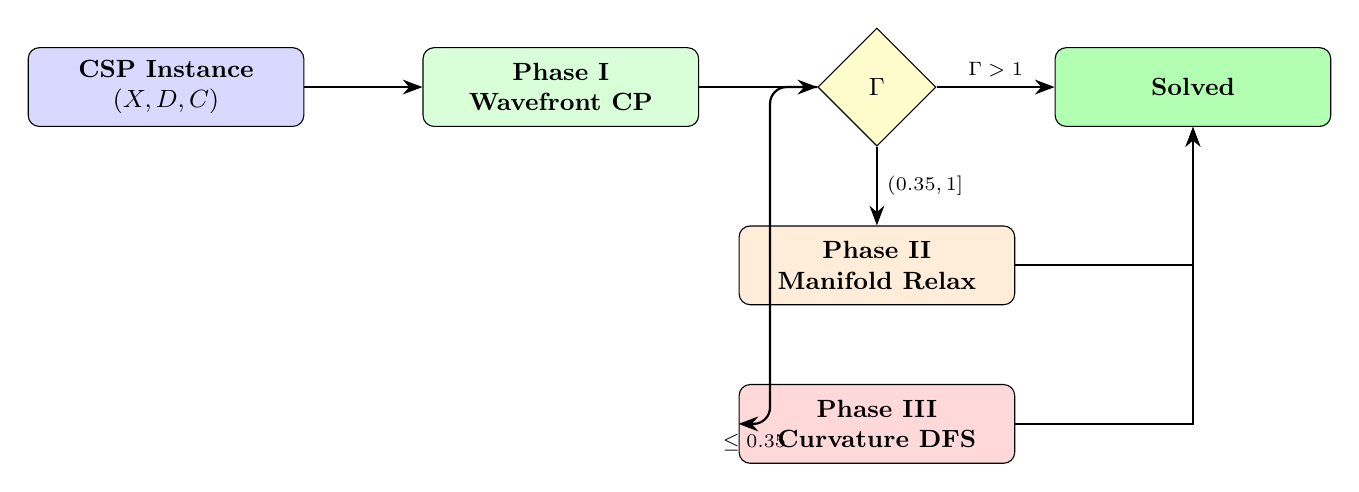
\begin{tikzpicture}[
    node distance=1.2cm and 1.8cm,
    phase/.style={draw, rounded corners, minimum width=3.5cm, minimum height=1cm, font=\small\bfseries, align=center},
    gate/.style={draw, diamond, minimum width=1.5cm, minimum height=1.5cm, font=\small, inner sep=1pt},
    arr/.style={-{Stealth[length=2.5mm]}, thick}
]
    % All instances enter Phase I first
    \node[phase, fill=blue!15] (input) {CSP Instance\\$(X, D, C)$};
    \node[phase, fill=green!15, right=1.5cm of input] (p1) {Phase I\\Wavefront CP};
    % Gamma gate comes AFTER Phase I
    \node[gate, fill=yellow!20, right=1.5cm of p1] (gamma) {$\Gamma$};
    \node[phase, fill=green!30, right=1.5cm of gamma] (solved) {Solved};
    % Medium path: Phase II (below, slight right)
    \node[phase, fill=orange!15, below=1cm of gamma] (p2) {Phase II\\Manifold Relax};
    % Hard path: Phase III (below Phase II, bypasses II)
    \node[phase, fill=red!15, below=1cm of p2] (p3) {Phase III\\Curvature DFS};

    % All instances flow through Phase I
    \draw[arr] (input) -- (p1);
    \draw[arr] (p1) -- (gamma);
    % Easy: Gamma > 1, solved by Phase I alone
    \draw[arr] (gamma) -- node[above, font=\scriptsize] {$\Gamma > 1$} (solved);
    % Medium: Phase II then solved
    \draw[arr] (gamma) -- node[right, font=\scriptsize] {$(0.35, 1]$} (p2);
    \draw[arr] (p2) -| (solved);
    % Hard: bypass Phase II, go directly to Phase III
    \draw[arr, rounded corners=6pt] (gamma.west) -- ++(-0.6,0) |- node[near end, below, font=\scriptsize] {$\leq 0.35$} (p3.west);
    \draw[arr] (p3) -| (solved);
\end{tikzpicture}
\caption{System architecture: Phase~I always executes first; the trichotomy parameter $\Gamma$ gates subsequent phases. Hard instances ($\Gamma \leq 0.35$) bypass Phase~II entirely.}
\end{figure}

% Figure 2: Constraint Fiber Bundle
\begin{figure}[h!]
\centering
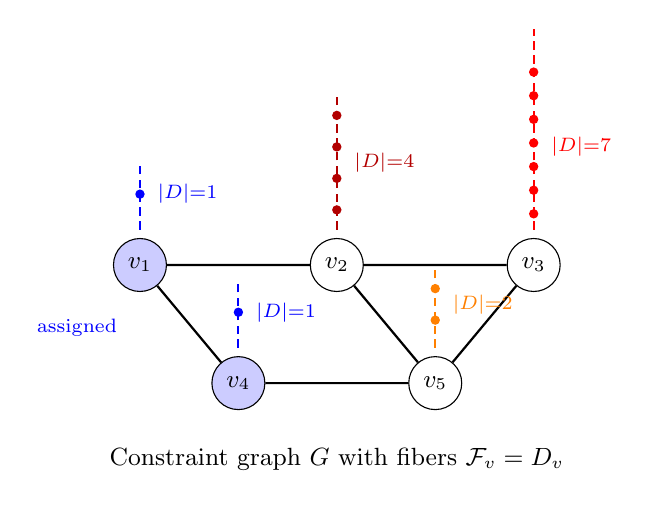
\begin{tikzpicture}[
    vertex/.style={circle, draw, minimum size=6mm, font=\small},
    fiber/.style={draw, thick, densely dashed},
    fiberpt/.style={circle, fill, inner sep=1.2pt}
]
    % Base graph
    \node[vertex, fill=blue!20] (v1) at (0,0) {$v_1$};
    \node[vertex, fill=white] (v2) at (2.5,0) {$v_2$};
    \node[vertex, fill=white] (v3) at (5,0) {$v_3$};
    \node[vertex, fill=blue!20] (v4) at (1.25,-1.5) {$v_4$};
    \node[vertex, fill=white] (v5) at (3.75,-1.5) {$v_5$};

    % Edges
    \draw[thick] (v1)--(v2) (v2)--(v3) (v1)--(v4) (v2)--(v5) (v4)--(v5) (v3)--(v5);

    % Fibers
    % v1: assigned (1 element)
    \draw[fiber, blue] (0, 0.45) -- (0, 1.3);
    \node[fiberpt, blue] at (0, 0.9) {};
    \node[font=\scriptsize, blue, right] at (0.1, 0.9) {$|D|{=}1$};

    % v2: 4 candidates
    \draw[fiber, red!70!black] (2.5, 0.45) -- (2.5, 2.2);
    \foreach \y in {0.7, 1.1, 1.5, 1.9} \node[fiberpt, red!70!black] at (2.5, \y) {};
    \node[font=\scriptsize, red!70!black, right] at (2.6, 1.3) {$|D|{=}4$};

    % v3: 7 candidates
    \draw[fiber, red] (5, 0.45) -- (5, 3.0);
    \foreach \y in {0.65, 0.95, 1.25, 1.55, 1.85, 2.15, 2.45} \node[fiberpt, red] at (5, \y) {};
    \node[font=\scriptsize, red, right] at (5.1, 1.5) {$|D|{=}7$};

    % v4: assigned
    \draw[fiber, blue] (1.25, -1.05) -- (1.25, -0.2);
    \node[fiberpt, blue] at (1.25, -0.6) {};
    \node[font=\scriptsize, blue, right] at (1.35, -0.6) {$|D|{=}1$};

    % v5: 2 candidates
    \draw[fiber, orange] (3.75, -1.05) -- (3.75, 0.0);
    \node[fiberpt, orange] at (3.75, -0.7) {};
    \node[fiberpt, orange] at (3.75, -0.3) {};
    \node[font=\scriptsize, orange, right] at (3.85, -0.5) {$|D|{=}2$};

    % Labels
    \node[font=\small, below] at (2.5, -2.2) {Constraint graph $G$ with fibers $\mathcal{F}_v = D_v$};
    \node[font=\scriptsize, blue] at (-0.8, -0.8) {assigned};
\end{tikzpicture}
\caption{Constraint fiber bundle $\pi: \mathcal{F} \to G$. Fiber dimension reflects domain size.}
\end{figure}

\clearpage

% Figure 3: Curvature Field (simplified)
\begin{figure}[h!]
\centering
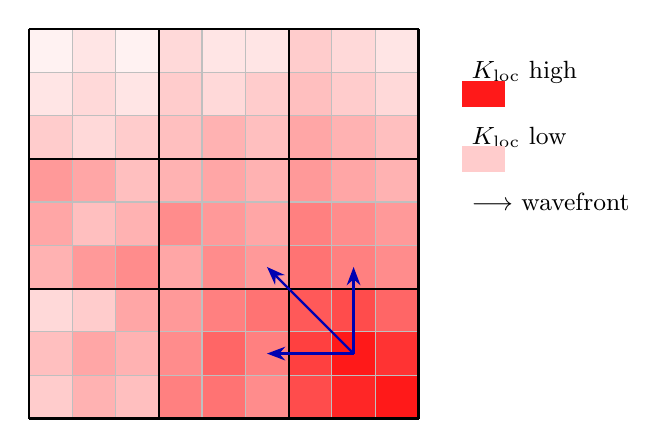
\begin{tikzpicture}[scale=0.55]
    % 9x9 grid with curvature heat map (manually set representative values)
    % Row 0 (bottom)
    \foreach \x/\v in {0/20, 1/30, 2/25, 3/50, 4/55, 5/45, 6/70, 7/85, 8/90} {
        \fill[red!\v!white] (\x, 0) rectangle (\x+1, 1);
    }
    \foreach \x/\v in {0/25, 1/35, 2/30, 3/45, 4/60, 5/50, 6/75, 7/90, 8/80} {
        \fill[red!\v!white] (\x, 1) rectangle (\x+1, 2);
    }
    \foreach \x/\v in {0/15, 1/20, 2/35, 3/40, 4/50, 5/55, 6/65, 7/70, 8/60} {
        \fill[red!\v!white] (\x, 2) rectangle (\x+1, 3);
    }
    \foreach \x/\v in {0/30, 1/40, 2/45, 3/35, 4/45, 5/40, 6/55, 7/50, 8/45} {
        \fill[red!\v!white] (\x, 3) rectangle (\x+1, 4);
    }
    \foreach \x/\v in {0/35, 1/25, 2/30, 3/45, 4/40, 5/35, 6/50, 7/45, 8/40} {
        \fill[red!\v!white] (\x, 4) rectangle (\x+1, 5);
    }
    \foreach \x/\v in {0/40, 1/35, 2/25, 3/30, 4/35, 5/30, 6/40, 7/35, 8/30} {
        \fill[red!\v!white] (\x, 5) rectangle (\x+1, 6);
    }
    \foreach \x/\v in {0/20, 1/15, 2/20, 3/25, 4/30, 5/25, 6/35, 7/30, 8/25} {
        \fill[red!\v!white] (\x, 6) rectangle (\x+1, 7);
    }
    \foreach \x/\v in {0/10, 1/15, 2/10, 3/20, 4/15, 5/20, 6/25, 7/20, 8/15} {
        \fill[red!\v!white] (\x, 7) rectangle (\x+1, 8);
    }
    \foreach \x/\v in {0/5, 1/10, 2/5, 3/15, 4/10, 5/10, 6/20, 7/15, 8/10} {
        \fill[red!\v!white] (\x, 8) rectangle (\x+1, 9);
    }

    % Grid lines
    \draw[gray!50] (0,0) grid (9,9);

    % Box boundaries
    \foreach \i in {0,3,6,9} {
        \draw[black, thick] (\i, 0) -- (\i, 9);
        \draw[black, thick] (0, \i) -- (9, \i);
    }
    % Wavefront arrows
    \draw[-{Stealth}, thick, blue!70!black] (7.5, 1.5) -- (5.5, 3.5);
    \draw[-{Stealth}, thick, blue!70!black] (7.5, 1.5) -- (7.5, 3.5);
    \draw[-{Stealth}, thick, blue!70!black] (7.5, 1.5) -- (5.5, 1.5);

    % Legend
    \node[font=\small, right] at (10, 8) {$K_{\mathrm{loc}}$ high};
    \fill[red!90!white] (10, 7.2) rectangle (11, 7.8);
    \node[font=\small, right] at (10, 6.5) {$K_{\mathrm{loc}}$ low};
    \fill[red!20!white] (10, 5.7) rectangle (11, 6.3);
    \node[font=\small, right] at (10, 5) {$\longrightarrow$ wavefront};
\end{tikzpicture}
\caption{Curvature field over 9$\times$9 constraint graph. Wavefront radiates from highest curvature.}
\end{figure}

% Figure 4: Trichotomy Phase Gating
\begin{figure}[h!]
\centering
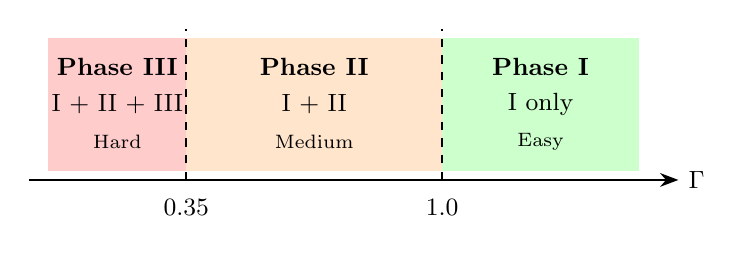
\begin{tikzpicture}[xscale=5, yscale=1.2]
    % Axis
    \draw[-{Stealth}, thick] (-0.05, 0) -- (1.6, 0) node[right, font=\small] {$\Gamma$};

    % Phase regions
    \fill[red!20] (0, 0.1) rectangle (0.35, 1.5);
    \fill[orange!20] (0.35, 0.1) rectangle (1.0, 1.5);
    \fill[green!20] (1.0, 0.1) rectangle (1.5, 1.5);

    % Boundaries
    \draw[thick, dashed] (0.35, 0) -- (0.35, 1.6);
    \draw[thick, dashed] (1.0, 0) -- (1.0, 1.6);

    % Labels
    \node[font=\small\bfseries] at (0.175, 1.2) {Phase III};
    \node[font=\small] at (0.175, 0.8) {I + II + III};
    \node[font=\scriptsize] at (0.175, 0.4) {Hard};

    \node[font=\small\bfseries] at (0.675, 1.2) {Phase II};
    \node[font=\small] at (0.675, 0.8) {I + II};
    \node[font=\scriptsize] at (0.675, 0.4) {Medium};

    \node[font=\small\bfseries] at (1.25, 1.2) {Phase I};
    \node[font=\small] at (1.25, 0.8) {I only};
    \node[font=\scriptsize] at (1.25, 0.4) {Easy};

    % Threshold labels
    \node[font=\small, below] at (0.35, -0.1) {$0.35$};
    \node[font=\small, below] at (1.0, -0.1) {$1.0$};
\end{tikzpicture}
\caption{Trichotomy phase gating: $\Gamma$ determines computational investment.}
\end{figure}

\clearpage

% Figure 5: GPU Execution Mapping
\begin{figure}[h!]
\centering
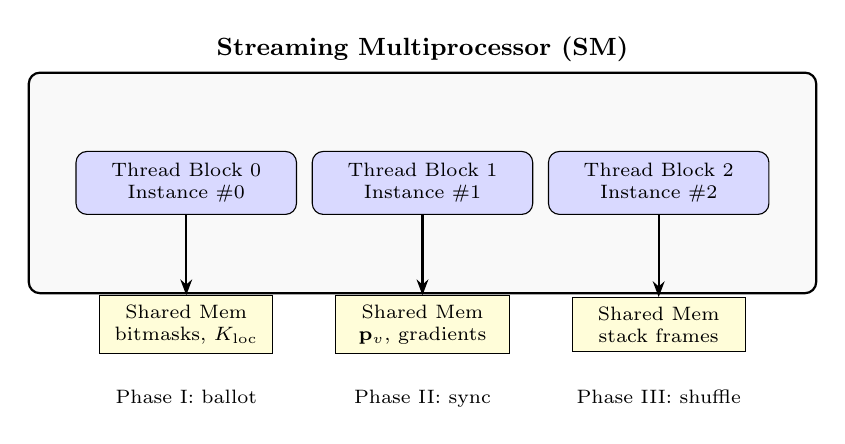
\begin{tikzpicture}[
    block/.style={draw, rounded corners, minimum width=2.8cm, minimum height=0.8cm, font=\scriptsize, align=center},
    smbox/.style={draw, thick, rounded corners, minimum width=10cm, minimum height=2.8cm, fill=gray!5},
    mem/.style={draw, fill=yellow!15, minimum width=2.2cm, minimum height=0.5cm, font=\scriptsize, align=center},
    arr/.style={-{Stealth[length=2mm]}, thick}
]
    % SM box
    \node[smbox] (sm) at (0, 0) {};
    \node[font=\small\bfseries, above] at (sm.north) {Streaming Multiprocessor (SM)};

    % Thread blocks
    \node[block, fill=blue!15] (tb1) at (-3, 0) {Thread Block 0\\Instance \#0};
    \node[block, fill=blue!15] (tb2) at (0, 0) {Thread Block 1\\Instance \#1};
    \node[block, fill=blue!15] (tb3) at (3, 0) {Thread Block 2\\Instance \#2};

    % Shared memory
    \node[mem] (sm1) at (-3, -1.8) {Shared Mem\\bitmasks, $K_{\mathrm{loc}}$};
    \node[mem] (sm2) at (0, -1.8) {Shared Mem\\$\mathbf{p}_v$, gradients};
    \node[mem] (sm3) at (3, -1.8) {Shared Mem\\stack frames};

    \draw[arr] (tb1) -- (sm1);
    \draw[arr] (tb2) -- (sm2);
    \draw[arr] (tb3) -- (sm3);

    % Warp label
    \node[font=\scriptsize, below] at (-3, -2.5) {Phase I: ballot};
    \node[font=\scriptsize, below] at (0, -2.5) {Phase II: sync};
    \node[font=\scriptsize, below] at (3, -2.5) {Phase III: shuffle};
\end{tikzpicture}
\caption{GPU execution mapping: one thread block per instance, one warp per block.}
\end{figure}

% Figure 6: Holonomy Pruning
\begin{figure}[h!]
\centering
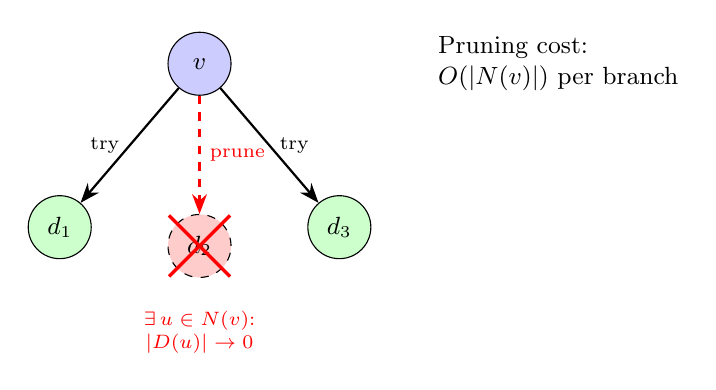
\begin{tikzpicture}[
    node distance=1.5cm,
    bnode/.style={circle, draw, minimum size=8mm, font=\small},
    pnode/.style={circle, draw, minimum size=8mm, font=\small, fill=red!20, dashed},
    arr/.style={-{Stealth[length=2.5mm]}, thick}
]
    % Branch point
    \node[bnode, fill=blue!20] (v) {$v$};

    % Branches
    \node[bnode, fill=green!20, below left=1.5cm and 1.2cm of v] (d1) {$d_1$};
    \node[pnode, below=1.5cm of v] (d2) {$d_2$};
    \node[bnode, fill=green!20, below right=1.5cm and 1.2cm of v] (d3) {$d_3$};

    \draw[arr] (v) -- (d1) node[midway, left, font=\scriptsize] {try};
    \draw[arr, red, dashed] (v) -- (d2) node[midway, right, font=\scriptsize, red] {prune};
    \draw[arr] (v) -- (d3) node[midway, right, font=\scriptsize] {try};

    % Singularity indicator
    \node[font=\scriptsize, red, below=0.3cm of d2, align=center] {$\exists\, u \in N(v)$:\\$|D(u)| \to 0$};

    % Cross out
    \draw[red, very thick] ($(d2.north west)+(-0.1,0.1)$) -- ($(d2.south east)+(0.1,-0.1)$);
    \draw[red, very thick] ($(d2.north east)+(0.1,0.1)$) -- ($(d2.south west)+(-0.1,-0.1)$);

    % Cost label
    \node[font=\small, right=2.5cm of v, align=left] {Pruning cost:\\$O(|N(v)|)$ per branch};
\end{tikzpicture}
\caption{Holonomy-based branch pruning: singularity detection eliminates dead branches.}
\end{figure}

\clearpage

% Figure 7: Throughput Scaling
\begin{figure}[h!]
\centering
\begin{tikzpicture}[xscale=0.9, yscale=0.35]
    % Axes (scale: 1 unit = 10K instances/sec)
    \draw[-{Stealth}, thick] (0,0) -- (11,0) node[right, font=\small] {Batch size ($\times 10^3$)};
    \draw[-{Stealth}, thick] (0,0) -- (0, 28) node[above, font=\small] {Throughput};

    % Grid
    \foreach \y/\l in {5/50K, 10/100K, 15/150K, 20/200K, 24.5/245K} {
        \draw[gray!30] (0,\y) -- (10.5,\y);
        \node[font=\scriptsize, left] at (0, \y) {\l};
    }
    \foreach \x/\l in {1/1,2/5,4/10,6/20,8/40,10/65} {
        \node[font=\scriptsize, below] at (\x, 0) {\l};
    }

    % Data curve (linear then saturate)
    \draw[blue, very thick] (1, 5) -- (2, 12) -- (4, 24.3) -- (6, 24.45) -- (8, 24.5) -- (10, 24.5);

    % Data points
    \foreach \x/\y in {1/5, 4/24.3, 10/24.5} {
        \fill[blue] (\x, \y) circle (3pt);
    }

    % Saturation line
    \draw[red, dashed, thick] (0, 24.5) -- (10.5, 24.5);
    \node[font=\scriptsize, red, right] at (10.5, 24.5) {245K/s};

    % Annotation
    \draw[-{Stealth}, thin] (5, 15) -- (4.2, 24);
    \node[font=\scriptsize, below right] at (4.5, 15) {SM saturation};
\end{tikzpicture}
\caption{Batch throughput scaling on RTX 5070. Saturation at $\sim$10K instances.}
\end{figure}

% Figure 8: Straggler Elimination
\begin{figure}[h!]
\centering
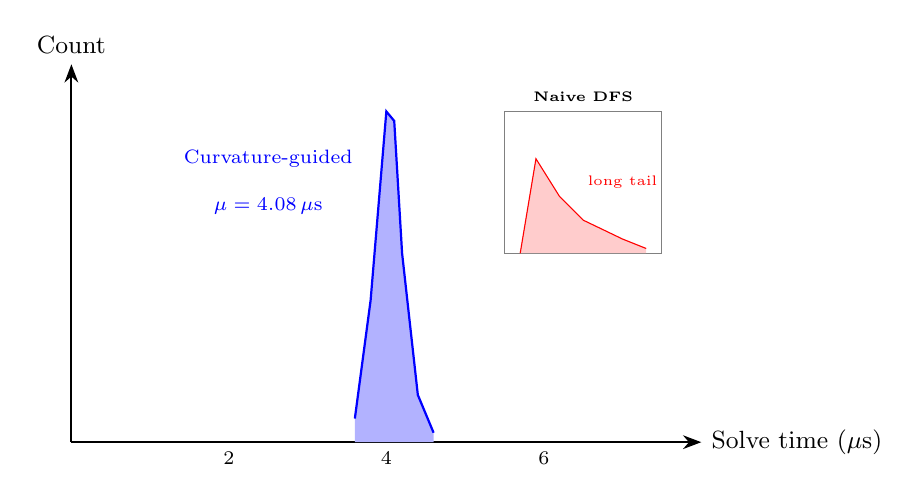
\begin{tikzpicture}[xscale=1.0, yscale=0.06]
    % Axes
    \draw[-{Stealth}, thick] (0,0) -- (8,0) node[right, font=\small] {Solve time ($\mu$s)};
    \draw[-{Stealth}, thick] (0,0) -- (0,80) node[above, font=\small] {Count};

    % Curvature-guided distribution (tight)
    \fill[blue!30] (3.6, 0) -- (3.6, 5) -- (3.8, 30) -- (4.0, 70) -- (4.1, 68) -- (4.2, 40) -- (4.4, 10) -- (4.6, 2) -- (4.6, 0) -- cycle;
    \draw[blue, thick] (3.6, 5) -- (3.8, 30) -- (4.0, 70) -- (4.1, 68) -- (4.2, 40) -- (4.4, 10) -- (4.6, 2);

    % Naive DFS label box (simplified inset)
    \draw[thin, gray] (5.5, 40) rectangle (7.5, 70);
    \node[font=\tiny\bfseries, above] at (6.5, 70) {Naive DFS};
    \fill[red!20] (5.7, 40) -- (5.9, 60) -- (6.2, 52) -- (6.5, 47) -- (7.0, 43) -- (7.3, 41) -- (7.3, 40) -- cycle;
    \draw[red, thin] (5.7, 40) -- (5.9, 60) -- (6.2, 52) -- (6.5, 47) -- (7.0, 43) -- (7.3, 41);
    \node[font=\tiny, red] at (7.0, 55) {long tail};

    % Labels
    \node[font=\scriptsize, blue] at (2.5, 60) {Curvature-guided};
    \node[font=\scriptsize, blue] at (2.5, 50) {$\mu = 4.08\,\mu$s};

    % Tick marks
    \node[font=\scriptsize, below] at (2, 0) {2};
    \node[font=\scriptsize, below] at (4, 0) {4};
    \node[font=\scriptsize, below] at (6, 0) {6};
\end{tikzpicture}
\caption{Straggler elimination: curvature-guided ordering (blue) vs.\ naive DFS (red inset).}
\end{figure}

% ====================================================================
% Empirical Data Figures (from actual GPU execution)
% ====================================================================

% Figure 9: Curvature Heatmap (actual data)
\begin{figure}[h!]
\centering
\includegraphics[width=0.55\textwidth]{01_curvature_heatmap.png}
\caption{Empirical curvature field $K_{\mathrm{loc}}(r,c)$ on a 15-clue extreme puzzle. Clue cells (grey) have $K = 0$. High-curvature cells cluster at the boundary of the assigned region.}
\end{figure}

% Figure 10: Throughput Scaling (actual data)
\begin{figure}[h!]
\centering
\includegraphics[width=0.65\textwidth]{05_gpu_throughput_scaling.png}
\caption{Measured batch throughput on 15-clue extreme Sudoku (RTX 5070). Saturation at $\sim$245K instances/sec confirms full SM occupancy with zero straggler penalty.}
\end{figure}

\clearpage

% Figure 11: Head-to-Head Benchmark (actual data)
\begin{figure}[h!]
\centering
\includegraphics[width=0.65\textwidth]{03_benchmark_comparison.png}
\caption{Head-to-head single-instance solve time (log scale). Davis GPU: 20.4~ms. DLX: 77.8~ms. CP: 3{,}066~ms. DFS: 4{,}195~ms. Davis CPU: 25{,}012~ms. The GPU achieves $1{,}226\times$ speedup over the CPU implementation of the same algorithm.}
\end{figure}

% Figure 12: Solve Composite (actual data)
\begin{figure}[h!]
\centering
\includegraphics[width=\textwidth]{08_solve_composite.png}
\caption{Four stages of the curvature-guided solve (steps 0, 15, 40, 66). Grey digits are clues; green digits are solver-placed. Background color encodes $K_{\mathrm{loc}}$. Curvature collapses monotonically.}
\end{figure}

\clearpage

% Figure 13: Energy Descent (actual data)
\begin{figure}[h!]
\centering
\includegraphics[width=0.7\textwidth]{09_energy_descent_static.png}
\caption{Energy descent during the 66-step solve. Top: Davis energy $E[\gamma]$ drops from 62.2 to 0. Middle: total curvature $\sum K$ collapses. Bottom: total entropy $\sum H$ drains as domains contract to singletons. No non-monotonic excursions.}
\end{figure}

\clearpage

\end{document}
